\documentclass[10pt,xcolor=pdflatex]{beamer}
\usepackage{newcent}
\usepackage[utf8]{inputenc}
\usepackage[slovak]{babel}
\usepackage{hyperref}
\usepackage{fancyvrb}
\usepackage{listings}
\usepackage{graphicx}
\usetheme{FIT}
\usepackage{siunitx}
\usepackage{pgfplots}

\pgfplotsset{compat=1.12}
\sisetup{
	round-mode          = places,
	round-precision     = 2,
}


\bibliographystyle{czechiso}


%%%%%%%%%%%%%%%%%%%%%%%%%%%%%%%%%%%%%%%%%%%%%%%%%%%%%%%%%%%%%%%%%%
\title{UnMasked}
\subtitle{Image inpainting}

\author{Eršek Martin [xersek00]\\ Hanzel Svätopluk [xhanze10]}

\institute{Brno University of Technology, Faculty of Information Technology}

\date{\today}

%%%%%%%%%%%%%%%%%%%%%%%%%%%%%%%%%%%%%%%%%%%%%%%%%%%%%%%%%%%%%%%%%%

\begin{document}

	\frame[plain]{\titlepage}
	
	\begin{frame}{UnMasked}
		\begin{itemize}
			\item UnMasked is a project aiming to remove face masks from peoples' faces using image inpainting
		\end{itemize}
	\end{frame}

	\begin{frame}{Solution}
		\begin{itemize}
			\item PyTorch\footnote{\url{https://pytorch.org/}}
			\item PyTorch Lightning\footnote{\url{https://www.pytorchlightning.ai/}}
			\item SN-PatchGAN \cite{yu2018free}
				\begin{itemize}
					\item Gated convolutions
				\end{itemize}
			\item CelebA-HQ dataset
				\begin{itemize}
					\item 30k images
				\end{itemize}
			\item on-the-fly masking using MaskTheFace\footnote{\url{https://github.com/aqeelanwar/MaskTheFace/}} \cite{anwar2020masked}
		\end{itemize}
	\end{frame}

	\begin{frame}{Results}
		\begin{figure}
			\centering
			\only<1>{
				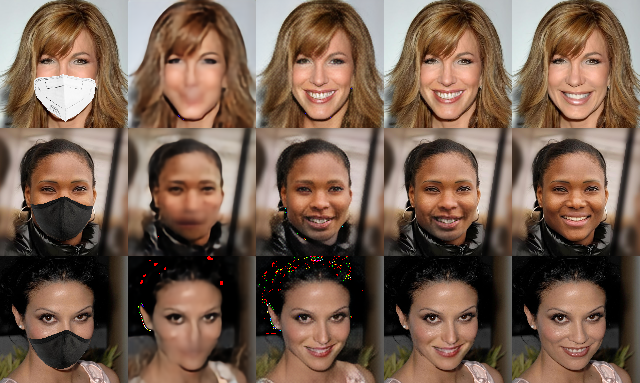
\includegraphics[width=0.7\linewidth]{img/unmasked-results1}
			}
			\only<2>{
				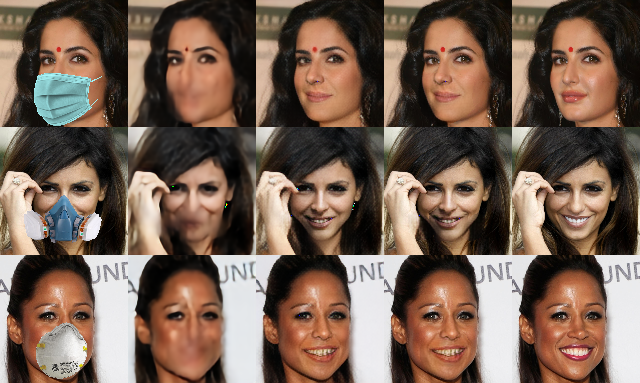
\includegraphics[width=0.7\linewidth]{img/unmasked-results2}
			}
			\caption{Network results from validation dataset. Left to right: input, coarse, refined, output, ground truth}
			\label{fig:unmasked-results}
		\end{figure}
	\end{frame}

	\begin{frame}{Results}
		\begin{figure}[h!]
			\begin{center}
				\begin{tikzpicture}
					\begin{axis}[
						width=\linewidth, height=5cm,
						grid=major,
						grid style={dashed,gray!30},
						xlabel=Skóre,
						ylabel=Počet,
						legend style={at={(0.5,-0.2)},anchor=north},
						xtick=data,
						ybar,
					]
						\addplot[blue, fill] table[x=score,y=count, col sep=comma] {user_research_male_csv};
						\addlegendentry{male}
						\addplot[red, fill] table[x=score,y=count, col sep=comma] {user_research_female_csv};
						\addlegendentry{female}
					\end{axis}
				\end{tikzpicture}
			
				\caption{
					Ohodnotenie vierohodnosti obrázka za pomoci užívateľského výskumu. X-ová os značí to ako veľmi realisticky vyzeral obrázok pre užívateľov. 1 - nerealistický, generovaný počítačom; 10 - originálna neupravovaná fotka
				}
				\label{user_research}
			\end{center}
		\end{figure}
	\end{frame}

	\begin{frame}{Conclusion}
		content...
	\end{frame}

	\bluepage{Thank you for your attention!}

	
	\begin{frame}{References}
		\nocite{*}
		\bibliography{references}
	\end{frame}
	
\end{document}
